%%%%%%%%%%%%%%%%%%%%%%%%%%%%%%%%%%%%%%%%%
% a0poster Landscape Poster
% LaTeX Template
% Version 1.0 (22/06/13)
%
% The a0poster class was created by:
% Gerlinde Kettl and Matthias Weiser (tex@kettl.de)
% 
% This template has been downloaded from:
% http://www.LaTeXTemplates.com
%
% License:
% CC BY-NC-SA 3.0 (http://creativecommons.org/licenses/by-nc-sa/3.0/)
%
%%%%%%%%%%%%%%%%%%%%%%%%%%%%%%%%%%%%%%%%%

%----------------------------------------------------------------------------------------
%	PACKAGES AND OTHER DOCUMENT CONFIGURATIONS
%----------------------------------------------------------------------------------------

\documentclass[a0,landscape]{a0poster}

\usepackage{multicol} % This is so we can have multiple columns of text side-by-side
\columnsep=60pt % This is the amount of white space between the columns in the poster
\columnseprule=3pt % This is the thickness of the black line between the columns in the poster

\usepackage[svgnames]{xcolor} % Specify colors by their 'svgnames', for a full list of all colors available see here: http://www.latextemplates.com/svgnames-colors

\usepackage{times} % Use the times font
%\usepackage{palatino} % Uncomment to use the Palatino font

\usepackage{graphicx} % Required for including images
\graphicspath{{figures/}} % Location of the graphics files
\usepackage{booktabs} % Top and bottom rules for table
\usepackage[font=small,labelfont=bf]{caption} % Required for specifying captions to tables and figures
\usepackage{amsfonts, amsmath, amsthm, amssymb} % For math fonts, symbols and environments
\usepackage{wrapfig} % Allows wrapping text around tables and figures

\usepackage{tcolorbox}
\usepackage{physics}
\usepackage{amsmath}
\DeclareMathOperator*{\argmin}{arg\,min} % thin space, limits underneath in displays

\begin{document}

%----------------------------------------------------------------------------------------
%	POSTER HEADER 
%----------------------------------------------------------------------------------------

% The header is divided into three boxes:
% The first is 55% wide and houses the title, subtitle, names and university/organization
% The second is 25% wide and houses contact information
% The third is 19% wide and houses a logo for your university/organization or a photo of you
% The widths of these boxes can be easily edited to accommodate your content as you see fit

\begin{minipage}[b]{0.88\linewidth}
\veryHuge \color{DarkSlateGray} \textbf{Explicit Non-Linear Dimensionality Reduction} \color{Black}\\ % Title
\huge \textbf{Pierre Visconti}\\ % Author(s)
\huge \text{Department of Mathematics,  Walla Walla University}\\
\end{minipage}
%
\begin{minipage}[b]{0.12\linewidth}

\includegraphics[width=13cm]{wwu.png} % Logo or a photo of you, adjust its dimensions here
\end{minipage}
%\vspace{1cm} % A bit of extra whitespace between the header and poster content

%----------------------------------------------------------------------------------------

\begin{multicols}{4} % This is how many columns your poster will be broken into, a poster with many figures may benefit from less columns whereas a text-heavy poster benefits from more

%----------------------------------------------------------------------------------------
%	INTRODUCTION
%----------------------------------------------------------------------------------------
\begin{tcolorbox}[colback=white,colframe=black]
    \color{DarkSlateGray}
    \begin{center}\section*{Introduction}\end{center}
\end{tcolorbox}
\color{Black}

Real world data is often complex and of high dimension. The high dimensionality of the data poses problems by the high computational cost in analyzing the data, and being difficult to understand. Dimensionality reduction is the idea that when the data is of artificially high dimension, it can be reduced to a lower dimension while still retaining the intrinsic properties of the data. Linear techniques such as Principal Components Analysis (PCA) have been well known for some time, but cannot handle complex non-linear data. Non-linear methods, known as Manifold learning, can handle complex data, however most existing algorithms do not build an explicit model, meaning new incoming data samples must be added to the original data and the dimensionality reduction algorithm run again on the entire dataset, thereby defeating the intended purpose of lowering the overall computational complexity. The goal of this project is to explore a manifold learning algorithm that builds an explicit model and apply it as a pre-processing step in supervised machine learning algorithms to reduce the overall time and storage complexity of the algorithm.\vspace{0.5cm}
%----------------------------------------------------------------------------------------
%	Background 
%----------------------------------------------------------------------------------------
\begin{tcolorbox}[colback=white,colframe=black]
    \color{DarkSlateGray}
    \begin{center}\section*{Background}\end{center}
\end{tcolorbox}
\color{Black}

\par Given a data set $\mathcal{X}:=\{x_1, x_2, ..., x_N\}$ in the high dimensional space $\mathbf{R} ^n$, assume there exists an explicit polynomial mapping from $\mathcal{X}$ to its low dimensional representation $\mathcal{Y}:=\{y_1, y_2, ..., y_N\}$ in $\mathbf{R}^m$. 
For a given data vector $x_i \in \mathcal{X}$, define the mapping $\phi:\mathbf{R}^n\rightarrow\mathbf{R}^{pn}$ as
\[\phi(x_i) =
\begin{bmatrix}
\overbrace{x_i \odot x_i \odot \cdots \odot x_i}^{p \text{ times}} \\
\vdots \\
x_i \odot x_i \\
x_i
\end{bmatrix}.\]
The $k$-th component of $y_i \in \mathcal{Y}$ is defined as a polynomial of degree $p$ with respect to $x_i$, such that
\[y_i^k = v_k^T\phi(x_i), \text{ where } v_k \in \mathbf{R}^{pn}\] 
\par The polynomial mapping assumption can then be combined with a popular dimensionality reduction algorithm known as Locally Linear Embedding (LLE). LLE aims to preserve local relationships between data points based on the idea that if the dataset is sampled from a smooth manifold, then the neighbors of each point remain nearby in the low-dimensional space. 
\par LLE first finds a set of linear coefficients that best reconstructs each data point $x_i$ by its $k$-nearest neighbors. Using Euclidean Distance, the linear reconstruction weights $R_{ij}, i,j=1,2,...,N$ are given by minimizing the sum of the squared distances between all the data points and their reconstructions, subject to the constraints that $x_i$ is only reconstructed from its neighbors, and the weights for $x_i$ must sum to 1. 
\[R_{ij} = \argmin_{\sum_{j=1}^N{R_{ij}}=1}\quad\sum_{i=1}^N{\norm{x_i - \sum_{j=1}^N{R_{ij}x_j}}}_{2}^2 \tag{i}\]
\par LLE then constructs a neighborhood preserving mapping by fixing the weights $R_{ij}$, while optimizing the coordinates $y_i$, subject to constraints that make the problem well-posed.
\begin{align*}
    \min{} \quad &\sum_{i=1}^N{\norm{y_i-\sum_{j=1}^N{R_{ij}y_j}}_2^2} \tag{ii}\\
    \\
    \text{s.t.} \quad &\frac{1}{N}\sum_{i=1}^N{y_iy_i^T=I_m}
\end{align*}
Applying the polynomial assumption to these concepts leads to the following algorithm.

\vspace{0.5cm}
%----------------------------------------------------------------------------------------
%	MATERIALS AND METHODS
%----------------------------------------------------------------------------------------
\begin{tcolorbox}[colback=white,colframe=black]
    \color{DarkSlateGray}
    \begin{center}\section*{Neighborhood Preserving Polynomial Embedding Algorithm}\end{center}
\end{tcolorbox}
\color{Black}
Given a data set $\mathcal{X}:=\{x_1, x_2, ..., x_N\}$ in the high dimensional space $\mathbf{R} ^n$, the NPPE algorithm finds an explicit polynomial mapping from $\mathcal{X}$ to its low dimensional representation $\mathcal{Y}:=\{y_1, y_2, ..., y_N\}$ in $\mathbf{R}^m$.
\vspace{1cm}
\subsection*{Algorithm Overview}
\textbf{Inputs:} Data matrix $X=[x_1 \hspace{0.5cm} x_2 \text{ }\cdots\text{ } x_N]$ of size $n \times N$, the number $k$ of nearest neighbors, the polynomial degree $p$, and the low dimensional space $m$. 
\begin{enumerate}
\item Compute the linear weights $R$.
\item Compute the non-linear weights $W$.
\item Solve the generalized eigenvalue problem to get the eigenvectors $v_i, i=1,2,...,m$.
\item Map the high-dimensional data to the low-dimensional embedding space.
\end{enumerate}
%------------------------------------------------
\subsection*{Computing the Linear Weights}
From Eq. (i), the linear weight matrix $R=\left[r_1 \hspace{0.5cm} r_2 \text{ }\cdots\text{ } r_N\right]$ in $\mathbf{R}^{N \times N}$, is given by computing the following closed formed solution for $r_i$, where $r_i$ is a column vector in the $i$-th row of $R$, $e$ is a column vector of all ones, and $G_{jl}=(x_j-x_i)^T(x_l-x_i)$ where $x_j,\,x_l$ are in the $k$-nearest neighbors of $x_i$. 
\begin{equation}
r_i = \frac{G^{-1}e}{e^TG^{-1}e}
\end{equation}
%------------------------------------------------
\subsection*{Computing the Non-linear Weights}
The non-linear weight matrix $W\in\mathbf{R}^{N\times N}$, is computed by the following equation. 
\begin{equation}
W_{ij} = R_{ij} + R_{ji} - \sum_{k=1}^{N}{R_{ik}R_{kj} \text{, and } D_i = \sum_{j=1}^N{W_{ij}}=1}
\end{equation}

%------------------------------------------------
\subsection*{Solving the Generalized Eigenvalue Problem}
Define $\phi = \left[\phi(x_1) \hspace{0.5cm} \phi(x_2) \text{ }\cdots\text{ } \phi(x_N)\right]$ to be a $(pn) \times N$ matrix and $W$ as the non-linear reconstruction weight matrix of size $N \times N$. Casting LLE into the framework of spectral embedding and applying the polynomial assumption turns Eq. (ii) into the following, where $D$ is a diagonal matrix with $i$-th entry $D_i$.
\begin{align*}
    \min_{v_k} \quad &\sum_{k}{v_k^T\phi (D-W)\phi v_k} \\
    \\
    \text{s.t.} \quad &v_j^T\phi D \phi v_k=\delta_{jk}
\end{align*}
By the Rayleigh-Ritz Theorem, the optimal solutions can be found by solving the following generalized eigenvalue problem to obtain the eigenvectors $v_i, i=1,2,...,m$ corresponding to the $m$ smallest eigenvalues. 

\begin{equation}
\phi(D-W)\phi^Tv_i = \lambda \phi D\phi^Tv_i, \quad v_i^T\phi D\phi^Tv_j=\delta_{ij}
\end{equation}

%------------------------------------------------
\subsection*{Mapping to the Low Dimensional Space}

For a data sample $x_i \in \mathcal{X}$, its low dimensional representation $y_i \in \mathcal{Y}$ is given by
\begin{equation}
y_i = \left[ v_1^T\phi(x_i) \hspace{0.5cm} v_2^T\phi(x_i) \text{ }\cdots\text{ } v_m^T\phi(x_i)  \right]^T
\end{equation}
Importantly, the mapping function above holds true for a new data sample $x_t \notin \mathcal{X}$, allowing for its low dimensional representation $y_t$ to be computed efficiently. 
%----------------------------------------------------------------------------------------
%	RESULTS 
%----------------------------------------------------------------------------------------
\begin{tcolorbox}[colback=white,colframe=black]
    \color{DarkSlateGray}
    \begin{center}\section*{Results and Conclusions}\end{center}
\end{tcolorbox}
\color{Black}

The NPPE algorithm is applied to the SwissRoll dataset comprised of points in $\mathbf{R}^3$, shown in \textbf{Figure 1}, to find an explicit polynomial mapping to $\mathbf{R}^2$. The data is split into a training set, the lower part, and a testing set, the upper part. The parameter of $k$-nearest neighbors is set to be $1\%$ of the training samples $N$ and the polynomial degree $p=2$.     

\begin{center}\vspace{1cm}
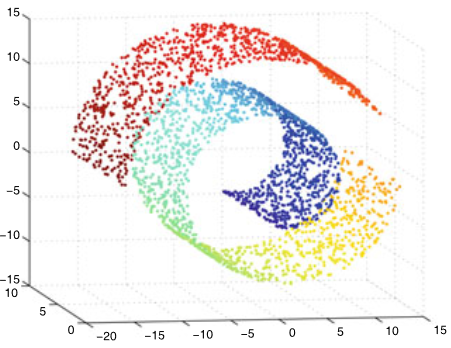
\includegraphics[width=0.8\linewidth]{figures/hd.png}
\captionof{figure}{\color{Black}{SwissRoll dataset in the high dimensional space $\mathbf{R}^3$}}
\end{center}\vspace{1cm}

The mapping relationship from $\mathbf{R}^3 \rightarrow \mathbf{R}^2$, computed by the NPPE algorithm, is performed only on the training set to test the performance on out of sample data. The learned mapping from the training set is used on both the training and testing sets to find their low dimensional representations, shown in \textbf{Figure 2}.
\begin{center}\vspace{1cm}
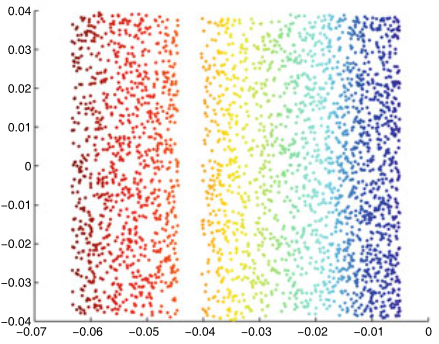
\includegraphics[width=0.8\linewidth]{figures/ld.png}
\captionof{figure}{\color{Black} Low dimensional representation of the SwissRoll dataset in $\mathbf{R}^2$}
\end{center}\vspace{1cm}
 \par Results show that the NPPE algorithm is effective at representing higher dimensional data in a low dimensional space. Importantly, the learned mapping function remains effective for samples not included in the original training set. 
 
%----------------------------------------------------------------------------------------
%	FORTHCOMING RESEARCH
%----------------------------------------------------------------------------------------

\begin{tcolorbox}[colback=white,colframe=black]
    \color{DarkSlateGray}
    \begin{center}\section*{Forthcoming Research}\end{center}
\end{tcolorbox}
\color{Black}
The implementation of the outlined NPPE algorithm, in C++ using Eigen3 for matrix operations and OpenMP for parallel computing, will be finalized. From there, the algorithm will be used as a pre-processing step to reduce the complexity of datasets for supervised machine learning algorithms and the lower overall computation time and hardware storage requirements will be measured. 
\vspace{0.5cm}

 %----------------------------------------------------------------------------------------
%	REFERENCES
%----------------------------------------------------------------------------------------

\begin{tcolorbox}[colback=white,colframe=black]
    \color{DarkSlateGray}
    \begin{center}\section*{References}\end{center}
\end{tcolorbox}
\color{Black}
\nocite{*} % Print all references regardless of whether they were cited in the poster or not
\bibliographystyle{plain} % Plain referencing style
\begingroup
\renewcommand{\section}[2]{} % Remove the title
\bibliography{sample} % Use the example bibliography file sample.bib
\endgroup
\textbf{Acknowledgements: } 
\par Research Advisor: Jonathan Duncan, PhD 
%----------------------------------------------------------------------------------------

\end{multicols}
\end{document}